\documentclass[conference]{IEEEtran}

\usepackage[utf8]{inputenc}
\usepackage[T1]{fontenc}
\usepackage[threshold=1]{csquotes}
\usepackage{xcolor}
\usepackage{framed}
\colorlet{shadecolor}{blue!20}

\ifCLASSINFOpdf
  \usepackage[pdftex]{graphicx}
  \graphicspath{{../images/}}
  \DeclareGraphicsExtensions{.pdf,.jpeg,.png}
\else
  \usepackage[dvips]{graphicx}
  \graphicspath{{../images/}}
  \DeclareGraphicsExtensions{.eps}
\fi

\begin{document}

\title{Engineering Privacy and Protest:\\a Case Study of AdNauseam}

\author{
  \IEEEauthorblockN{Daniel C. Howe}
  \IEEEauthorblockA{School of Creative Media\\City University, Hong Kong\\Email: daniel@rednoise.org} \and
  \IEEEauthorblockN{Helen Nissenbaum}
  \IEEEauthorblockA{Cornell Tech\\New York University\\Email: hfn1@nyu.edu}
}

\maketitle

\emph{Abstract}---The strategy of obfuscation has been broadly applied---in search, location tracking, private communication, anonymity---and, as such, has been recognized as an important element of the privacy engineer's toolbox. However, there remains a need for clearly articulated case studies describing not only the engineering of obfuscation mechanisms but, further, providing a critical appraisal of obfuscation's fit for specific socio-technical applications. This is the aim of our paper, which presents our experiences designing, implementing, and distributing AdNauseam, an open-source browser extension that leverages obfuscation to frustrate tracking by online advertisers.\\
\indent At its core, AdNauseam works like a list-based blocker, hiding or blocking ads and other trackers. However, it provides two additional features. First, it collects each ad that it finds in its ‘Vault’, allowing users to interactively explore the ads they have been served, and providing insight into the algorithmic profiles created by advertising networks. Second, AdNauseam simulates clicks on ads with the intention of confusing trackers and diminishing the value of aggregated tracking data.\\
\indent A critic might ask: why click? Why not simply hide ads from users and hide users from trackers? The twofold answer reveals what may be distinctive elements of the AdNauseam approach. To begin, we conceptualize privacy as a societal value. Whereas many privacy tools offer solutions only for individual users, AdNauseam is built on the assumption that, often, effective privacy protection must be infused throughout a system. This assumption presents different and interesting engineering challenges. Second, AdNauseam seeks to concurrently achieve the goal of resistance through protest. And since protest frequently involves being vocal, AdNauseam's core design conflicts at times with conceptions of privacy based on secrecy or concealment. While such tensions, and the tradeoffs that result, are not uncommon in privacy engineering,  the process of designing and building AdNauseam demanded their systematic consideration and resolution.\\
\indent In this paper we present the challenges we faced in attempting to apply obfuscation to a new domain, that of online tracking by advertisers. We begin with the goals of the project and the implemented features to which they were mapped. We then present the engineering approach employed and the tensions that arose during implementation, as well as the ways in which these tensions were resolved. We discuss our early attempts at evaluation on both technical and ethical dimensions, and present issues of distribution, including Google's ban of AdNauseam from its Chrome store. We conclude with thoughts on the broader challenges facing privacy tools which must operate within complex socio-technical contexts, especially those dominated by actors openly resistant to them.


\section{Introduction}

% no \IEEEPARstart
The ad blocking wars \cite{Murphy} reflect wide ranging resistance to aspects of the online advertising landscape, specifically tracking, malware, annoyance, degradation of browser performance, and bandwidth costs. A number of technical systems, utilizing diverse techniques, have addressed these issues in various combinations. AdNauseam, an open-source, cross-platform browser extension, contributes to this growing arsenal by leveraging obfuscation in an attempt to frustrate those seeking to profile users based on interests revealed through ad clicks. Specifically AdNauseam enables users to click discovered ads behind the scenes in order to register visits in ad network databases. The aim of the software is to pollute the data gathered by trackers and, by diminishing confidence in this  indicator, render their efforts to profile less effective and less profitable. At the same time, the software allows users to engage in a form of expression, by actively disrupting the economic system that drives surreptitious tracking, and by creating mistrust (advertisers generally pay ad networks for clicks) within the advertising system. Additionally, AdNauseam makes the ads it collects available to users to explore at their convenience, via interactive displays that update in real-time.

\subsection{Engineering Philosophy}

Our approach to the development of AdNauseam builds on prior work that has explicitly taken social values into consideration during tool design \cite{Friedman,Flanagan,Howe-1}. Throughout planning, development, and testing phases, we have integrated values-oriented concerns as first-order “constraints” together with more typical engineering metrics such as efficiency, speed, and robustness. Specific instances of values-oriented constraints include \emph{visibility and transparency} in interface, function, code, process, and strategy; \emph{personal autonomy}, where users need not rely on third parties; \emph{social protection of privacy} with distributed/community-oriented action; \emph{minimal resource consumption} (cognitive, bandwidth, client and server processing); and \emph{usability} (size, speed, memory consumption, configurability, and ease-of-use). Enumerating values-oriented constraints early in the design process enables us to iteratively revisit and refine them in the context of specific technical decisions. Where relevant in the following sections, we discuss ways in which AdNauseam benefited from this values-oriented approach, as well as tensions between design goals that emerged. Additionally we have followed a number of strategies from the literature on privacy-by-design \cite{Gurses-0, Hoepman, Gurses-1, Hansen, Cavoukian} by including \emph{Data Minimization Strategies}, \emph{Legitimacy Analysis} and \emph{Socially-informed Risk Analysis} as elements of our design process.

\subsection{Design Goals and Constraints}

The AdNauseam extension attempts to realize three tangible goals for the context of online tracking via advertising. The first is to offer \emph{protection}; protection against for users against malware and “malvertising” (malicious software that leverages advertising mechanisms to gain access to users' systems \cite{Mansfield}), as well as protection against data aggregation and profiling (either for individual users, the aggregate set of users, or both)  via clicks on advertisements. The second goal is to provide a means of proactive engagement, allowing users an avenue for \emph{expression} of their dissatisfaction with current advertising mechanisms to those in control of such systems. In the case of AdNauseam, this expression has an interventional aspect, as the software actively attempts to disrupt the economic model that drives advertising surveillance. The third goal is to facilitate \emph{transparency} regarding the advertising ecosystem---and the profiling on which it operates---by providing users with the ability to view the ads they are served in real-time, and later, to explore interactive visualizations of the ads collected over time, providing a rare glimpse of how advertisers view them. These mechanisms are augmented by in-interface links to additional learning resources.

\subsection{Social-Technical Context}

AdNauseam applies obfuscation to the context of tracking and profiling by online advertisers. If we compare this context to others where obfuscation has been applied (e.g., search), we notice both similarities and differences. In both cases users are confronted with large corporate entities (search engines and advertising networks) whose business models depend on the bulk collection of personal data. And in both cases users have little say in these interactions; the only alternative is to fully opt-out and abandon use of the service. While this may be an option in the case of search (by, for example, switching to a non-tracking engine like DuckDuckGo), one would have to stop, for the most part, using the web itself to opt-out of advertising surveillance, which for most users is not a realistic option. \footnote{Thus, from this perspective at least, obfuscation may be more legitimate for the advertising case than the search case, due to the lack of viable alternative options, a point discussed further below.} A second difference is the degree to which users want the service provided by the trackers. For search, we can assume that most users do in fact want (or need) the service offered by the search engine. For advertising networks, this is not as clear. Tracking aside, some subset of users may find ads useful, while another would prefer not to see ads at all; while a third might tolerate non-tracking ads only to avoid subscription fees. A third difference is that in search there is a single adversary (the search engine) with a high degree of knowledge, including prior search queries, interest profile(s), click frequency, timing data, etc. However, in advertising we are faced with multiple actors (ad-hosting web sites, advertisers, trackers, advertising networks, etc.), each of which interacts with the user in different ways, and is privy to different aspects (and data) of those interactions.

\subsection{Feature Mapping}

The mapping of goals to features (and to the system modules described below) was performed as follows: The goal of \emph{protection} was implemented at a basic level by the clicking of collected ads, via the visitation module; and by the blocking of non-visual trackers and other malware, via the detection module. The former attempts to protect the user from data profiling via clicks on advertisements, and the latter from non-visual tracking and potential malware. \emph{Expression} was realized through clicks, again via the visitation module, and also in our implementation of the EFF's Do Not Track (DNT) mechanism \cite{EFF-1}. With DNT enabled (the default setting), the DNT header is sent with all requests, and ads on DNT sites remain visible. Ads on these DNT pages are also not visited by AdNauseam. The goal of increased \emph{transparency} is realized through the visualization module, specifically via the real-time menu interface, where users can watch as new ads are discovered, then visited; the vault interface (described below), and a range of explanatory links embedded throughout AdNauseam's settings pages. Additionally, an in-depth Frequently-Asked-Questions (FAQ) list is linked from multiple locations within the interface.

\subsection{Data Minimization}

Following a growing body of literature on privacy-by-design \cite{Gurses-0, Hoepman, Gurses-1, Hansen, Cavoukian}, our design and implementation process followed principles of data minimization. Thus AdNauseam was designed to function without ever communicating to a “home server” or sending user-data to any other entity, for any reason. For developers, this meant we were unable to access usage patterns and related data, which may have yielded important insights. Yet this both clarified our own position in regard to data collection, and also enabled us to sidestep potential problems of data leakage or interception in transit.

% Similarly, this principle helped us to identify three pieces of private information which could potentially be leaked during normal function of the tool, and to then expose these as user options, with defaults that would provide normal users with full protection, while allowing advanced users the option to change these settings for higher performance. These data were all potentially exposed to third-parties (websites and advertising networks) as part of the normal HTTP headers sent with requests for ads being clicked; specifically page referer, user-agent, and cookies. From either the referer or cookies, an advertising network present on multiple sites (Google, for example, is estimated to have code running on 70\% of websites \cite{Englehardt}) could potentially recreate large portions of a user's click path, while the user-agent header could be used by malicious trackers attempting to perform browser fingerprinting \cite{Nikiforakis}. Thus all such information was stripped from outgoing requests by default. As discussed below, this choice is not without consequences. Choosing to foreground the safety of user data in this way impacted AdNauseam's efficacy on other goals.

\vspace{2mm}
\blockquote{\emph{The application of data minimization does not necessarily imply anonymity, but may also be achieved by means of concealing information related to identifiable individuals} \cite{Gurses-0}.}
\vspace{1mm}

\noindent Additionally we have applied the principle of data minimization to our ad export feature, which allows users to export their aggregate ad collection (as JSON) in order to sync or migrate between machines, to backup, or to share. From our experiences user-testing this feature, we noted that such exports contained potentially sensitive data, specifically users' click trails (stored as the locations for found ads), possibly over months or even years. When considering how to handle this data we noted that it also existed in the browser's local storage, which could potentially be accessed by a malicious actor. Thus we subsequently implemented encryption for this data, both in memory and in storage, as well as offering the user the option, before each export, to redact ad locations if desired.

\subsection{Legitimacy Analysis}

\vspace{1mm}
\blockquote{\emph{Before any privacy-by-design activities are embarked upon, a discussion needs to take place with respect to the “legitimacy” of the desired system given its burden on privacy. Legitimacy is described as “the establishment that the application goals would be useful for the intended use population.”}\cite{Iachello}\cite{Gurses-1}}
\vspace{1mm}

\noindent{A critic might ask: why click? Why not simply hide ads from users and hide users from trackers? There are two reasons. First, AdNauseam is inspired by the path-breaking work of Priscilla Regan, who argues that beyond the protection of individual interests, privacy may serve social ends, similar to collective goods such as clean air or national defense \cite{Regan}. This notion of privacy as a collective good presents interesting engineering and evaluation challenges, which, in our view, warrant close attention. Thus AdNauseam may stimulate deliberation not only on its particular features, but may draw attention to the conception of privacy it seeks to promote. A second reason for clicking, as opposed to simply blocking, is that AdNauseam seeks concurrently to achieve the goal of expressive resistance to tracking through protest. And since protest generally involves being vocal, AdNauseam's design seeks to give voice to users. Rather than enacting privacy as concealment, AdNauseam provides a means for users to express, in plain sight, their dissent by disrupting the dominant model of commercial surveillance. This approach embodies a principle drawn from the theory of contextual integrity, namely, privacy as appropriate flow of information\cite{Nissenbaum}. Thus, AdNauseam does not hide deliberate clicks from trackers but rather, by surrounding these clicks with decoy clicks, obfuscates inferences from clicks to users’ interests, which may be manipulated in various ways, including via behavioral advertising. AdNauseam does not block clicks; instead it blocks inappropriate access to interest profiles that trackers may infer from them.}

\indent Some have argued that simply using a quality ad blocker offers similar degrees of protection and expression. And while basic ad blocking does protect the individual user to a large degree, it does little to protect those without the resources (whether knowledge, free-time, or technical expertise) to find, install, and configure an ad blocker, let alone to verify that it works as it claims to. Thus, we argue, there is a need for tools which work to provide protection beyond the individual user (for the case of AdNauseam, both by attempting to polluting the aggregate data set and reduce its value to profilers, and by bringing attention to the problematic behavior of such advertisers). Similarly, while blocking may also realize expressive results (as evidenced by the frequency of media reports in which advertisers “respond” to the increased use of ad blockers), the nature of this expression is different from that of AdNauseam's approach. This difference is apparent in the intentional component of the expression: the advertising industry generally interprets ad blocker use as a critique of the aesthetic quality of ads, while they may read AdNauseam's expression instead as a critique of an ethically compromised industry\footnote{This is our intent at least; Google's recent ban of the software may imply that this intent is understood.}. Further, we see a difference in the qualitative \emph{experience} of tools users, a concern beyond the scope of this paper, but one that we return to briefly in \emph{Future Work}.

% \indent As discussed below, depending on the click-probability setting chosen by the user, AdNauseam's obfuscating activity may be apparent to advertising networks via increased click frequency (or even via pushback from advertisers contesting charges for software-generated clicks). Assuming that it is detected, we may still note technical differences between  the use of an ad blocker may often be transparent to a first-party website, it is not, unless special measures are taken, equally apparent to ad networks or advertisers. If we consider the general scenario in which a real-time auction is held for each display ad, we must consider at least three distinct cases, based on the type of blocking that occurs. First, if the entire DOM element containing the ad is blocked (e.g., a DIV or IFRAME), then no auction for that space occurs, and the ad network is, most likely, unaware even of the page view. No ad is created and no advertisers are involved. Second, if the auction is allowed to occur, and an advertiser chosen, and the request to that advertiser is then blocked, then the advertiser may be aware of the block, but it is not clear that the ad network would be. In the third case, where the auction occurs and the ad content is downloaded and then hidden by the ad blocker (as happens on nearly all search pages), it unclear that any of the aforementioned parties (including even the first-party website) would be aware of the block.

\indent Finally, critics have claimed that AdNauseam harms “independent content producers who can no longer support their sites.” As this critique touches a broad array of tools, including standard ad blockers, it will take us too far afield to address it fully here. However, setting aside the rejoinder which points out that these sites are enabling surveillance, or more harshly, “selling out” their visitors, the hope is that loosening the chokehold of tracking over web and mobile domains will allow other business models to flourish. Toward this end we have enabled support in AdNauseam for the EFF's DNT mechanism, a machine-verifiable, and potentially legally-binding, assertion on the part of sites that commit to privacy-respecting behavior \cite{EFF-1}. For sites that make this commitment, AdNauseam does not (by default) hide, block, or click their ads.

\subsection{Socially-informed Risk Analysis}

Given the goals we hoped to achieve and the set of features to which these mapped, we set out to identify risks to which users might be exposed. For each such risk, we considered the degree to which the user would be exposed when browsing the web using an unmodified browser, in comparison to the degree of exposure while using AdNauseam. Finally we considered their exposure using existing alternatives, ad-blockers like AdBlock Plus \cite{AdBlock} or wide-spectrum blockers like uBlock \cite{Gorhill}(see, for example, Figure \ref{fig:thirdparty} below). The following risks were identified:
% increased tracking by advertisers, leakage of personal data; and harms via malware/malvertising.

\vspace{2mm}
\begin{itemize}
\item Increased tracking by advertisers and other data-gatherers
\item Personal data leakage (via clicks, via hiding rather than blocking, via ad export)
\item Harms via malware or “malvertising”
\end{itemize}
\vspace{1mm}


\noindent To establish a lower-bound on exposure, we imposed a constraint that user exposure with AdNauseam must be strictly lower on all dimensions than with our baseline case of browsing with an unmodified browser. Conversely, we hypothesized that the current performance of uBlock, the open-source blocker with the best performance metrics, would provide an upper-bound on risk exposure for the individual user. As AdNauseam must interact, at least minimally, with advertising servers in order to fulfill its functional requirements, it would necessarily expose users to more risk than the current state-of-the art blocker. Notice that we refer specifically here to risk for \emph{the individual}, a distinction we return to below. In all cases noted above (see \emph{Comparative Evaluation} below), we were able to verify that risk to users was diminished with AdNauseam, both in comparison with the no-blocker case, \emph{and} to AdBlock Plus, the most commonly installed blocker\cite{PageFair}.

\section{Architecture}

The AdNauseam software is comprised of four modules, each responsible for one of its primary functions: detection, extraction, visualization, and visitation.

\subsection{Detection}

This module is responsible for the analysis and categorization of requests following a page view. Such requests, most often to third-parties, are first classified according to the type of elements they realize; whether advertisements, analytics, beacons, social-media, or functional widgets. The largest proportion of such requests (40-50\%) are made to the first group, on which this module focuses, which includes ad and ad-tracking services \cite{Wills}. This module determines which requests to block and which to allow, and distinguishes, in the latter category, between those that yield visual elements and those used only for tracking.

In order to categorize such requests, we leverage the capabilities of the open-source uBlock-Origin \cite{Gorhill} project, a configurable, list-based “blocker” that is effective and efficient \cite{Wills}. Like other blockers, uBlock allows users to specify publicly accessible lists of resources which contain syntactic matching rules for the retrieval of web resources. Based on these lists, we first determine whether a request should be blocked or allowed, and then, if allowed, whether it should be visible or hidden. If hidden, the element is downloaded and included in the page, but made invisible to the user via a content-script. Both blocking and hiding are specified via rules that may include the serving domain, the type of resource (e.g., images or video), and/or properties of the DOM container (for example, a DIV with a specific id or class). Rules are included from widely distributed lists that are updated and maintained by individuals and communities (e.g, “EasyList“ \cite{EasyList}. Additionally, users can augment these lists with custom rules they create, either to block or hide new content, or to whitelist a site, page, or element.

Requests marked as blockable in AdNauseam are disallowed at the network level, mimicking the behavior of most other blockers, including uBlock, AdBlock Plus, Adblock, and Adguard, which perform blocking on some percentage of requests, and hiding on the remainder. The difference for AdNauseam is that a subset of requests which might be blocked in other blockers must be allowed in AdNauseam; specifically those that result in visual advertisements.\footnote{Interestingly, it is exactly this standard combination of functions---hiding and blocking---that Google cites as being in violation of its Terms of Service, a claim discussed below in the \emph{Distribution} section.} At the element hiding level, the detection module is invoked incrementally, via content-scripts, as page elements are loaded (or dynamically generated) and inserted into the DOM. Elements marked for hiding are assigned a CSS class that sets their display to invisible, and the surrounding DOM is collapsed so as not to leave blank space on the page. Each hidden element (generally a visual ad) is then passed to the \emph{Extraction} module.


\subsection{Extraction}

Once a visual element has been detected and hidden, we must then determine whether it is in fact an advertisement. If so, the extraction module of the system must extract the properties needed by the \emph{Visualization} and \emph{Visitation} modules. These properties include timestamp, size, content-URL, target-URL, page-detected-on, etc. Text-only ads, as often found on search engines, present a different challenge, as these are generally served inline along with page content rather than requested from a 3rd-party server. In these non-image cases, several additional fields are aggregated to form the content payload (title, description, tagline) and there is no content-URL linking to an external resource. To enable extraction of such data, AdNauseam includes a custom set of CSS selectors used to parse specific DOM attributes from text-ad sites (Google, Ask, Bing, etc.). Such filters run only on specific domains where text-ads have been previously discovered.


\subsection{Visualization}

In order to facilitate transparency regarding tracking and profiling by advertisers, AdNauseam provides users with interactive visualizations of their collected ad data. These visualizations provide both high-level displays of aggregate data (see Figure \ref{fig:vault}), as well as the option to inspect individual ads (see Figure \ref{fig:inspector}) for data including the page on which the ad was found, the target URL, the text copy, the viewed-on date, ad network, and image or video ‘content’. Additionally, a number of derived functions provide additional metrics (i.e., the total estimated charge to advertising networks for the ads visited on a given page or in a given time-period, as in Figure \ref{fig:menu}). Ads may be filtered and sorted according to a variety of criteria: by date, topic-category, ad-network, page-category, etc. The visualization module is a distinct contribution of AdNauseam that attempts to a) provide users with greater insight concerning their interactions with advertisers, and b) enable interested users and researchers to study the ad data collected. To facilitate the latter, we include mechanisms for importing and exporting ad data sets, which can be loaded and saved as plain-text JSON files directly from the extension. The use of this data, aggregated across users, for further research (with appropriate mechanisms for user consent) is an area of future work.

\begin{figure}[!t]
\centering
\includegraphics[width=2.5in]{images/vault.png}
\caption{AdNauseam's AdVault visualization.}
\label{fig:vault}
\vspace{2mm}
\includegraphics[width=2.5in]{images/inspector.png}
\caption{Inspecting a single ad in the AdVault.}
\label{fig:inspector}
\vspace{2mm}
\includegraphics[width=2.5in]{images/menu.png}
\caption{Estimated cost to advertising networks.}
\label{fig:menu}
\end{figure}


\subsection{Visitation}

This module simulates clicks (or visits) on collected ads, with the intention of appearing to the serving website (as well as to advertisers and ad networks) as if the ad had been manually clicked. Currently, these clicks are implemented via AJAX, which simulates requests (matching headers, referer, etc.) that the browser would normally send. This provides users with protection against potential malware in ad payloads, as responses are not executed in the browser, and JavaScript, Flash, and other client-side scripting mechanisms are not executed. Similarly, AdNauseam blocks incoming cookies in responses to ad visits. The likelihood that a particular ad will be clicked depends on the user-configurable click-probability setting described further below.

What are the expected results of visiting some percentage of each user's collected ads? First, the data profiles of these users stored by advertising networks and data brokers may be polluted, as users' actual interests are hidden by generated clicks. This both protects individual users (assuming they have clicked, or may click, some ad in the future) as well as the larger user community, as aggregate statistics are less accurate and thus less valuable. Second, as advertisers must now potentially pay publishers for decoy clicks, a degree of mistrust is introduced into the economic model that drives the system. This is perhaps the most compelling argument for this strategy, as it could, given adequate adoption, force advertisers to change their behavior, either by developing new algorithms to filter such clicks, and/or by adopting more privacy-friendly policies (e.g., the EFF's Do Not Track mechanism).

\subsection{Distribution}

Although not often discussed in an engineering context, issues surrounding the distribution of AdNauseam highlight concerns we imagine will become only more relevant as corporate players exert a growing influence over the software ecosystem.

The prototype for AdNauseam was initially developed as a Firefox-only extension available in  Mozilla's addon store. In our production release, we added Opera and Chrome support and made the extension available in the Opera and Chrome stores respectively. We distributed upwards of 50,000 copies of the software over the subsequent six months, with the majority via Google's Chrome store. In January of 2017 however, we learned that Google had banned AdNauseam from the store, and further, had begun disallowing even manual installation or updates, effectively locking users out of their own saved data, all without prior notice or warning.

We wrote to Google requesting justification for the removal, and they responded that AdNauseam had breached the Store's Terms of Service, stating: “An extension should have a single purpose that is clear to users.”\footnote{In the one subsequent email we received, a Google representative stated that a single extension should not perform “both blocking and hiding,” an assertion that is difficult to accept at face value as nearly all ad blockers (including uBlock, AdBlock Plus, Adguard, etc.) perform blocking and hiding, and have not thus far been banned.} The single purpose of AdNauseam, we would argue, is not at all unclear---namely to resist the non-consensual surveillance conducted by advertising networks, of which Google is a prime example. Of course we understand that Google would prefer users not to install AdNauseam, as it opposes their core business model, but the Terms of Service do not (at least thus far) require extensions to endorse Google's business model. Moreover, this is not the justification cited for the removal. Whether or not one is an advocate of obfuscation, it is disconcerting to know that Google can make a privacy extension, along with stored data and preferences, disappear without warning. In this instance it is a counter-surveillance tool that is banned. Perhaps tomorrow it will be a secure chat app, or password manager. For developers, who, incidentally, must pay a fee to post items in the Chrome store, this should be cause for concern. Not only can one's software be banned without warning, but all comments, ratings, reviews, releases and statistics are removed as well.


\section{Design Tensions}

\subsection{Indistinguishability and Protection}

For obfuscation to function effectively as a means of counter-surveillance, the noise generated must exhibit a high degree of \emph{indistinguishability} with regards to data the system intends to capture; that is, it must be difficult for an adversary to distinguish injected noise from the data it is attempting to collect \cite{Gervais}. However, there are times when this goal comes into tension with other aims of the software, specifically that of protection, e.g., from malware.

For example, after issuing a software-generated click on an ad, we must decide whether the DOM for the response should be parsed and executed, and whether client-side scripts should be allowed to run. In current AdNauseam versions, visits are implemented via AJAX requests, which means that a DOM is not constructed from the response, and client-side scripts are not executed. While protection is maximized here (against malicious code embedded in ads, i.e., malvertising), obfuscatory power may be diminished. For example, one vector of attack we have noted is from an adversary who, upon receiving a click request, sends a preliminary response containing JavaScript code that executes from within the DOM to issue the actual request for the ad's target. In this case, if the client-side code in the preliminary response never runs, then, from the advertising network's perspective, the click is never executed. We have experimented with solutions that address this issue and thus better support indistinguishability (including executing clicks in sandboxed invisible tabs), but have yet to settle on a cross-platform solution that adequately protects user from potential malware/malvertising. For the moment we leave this as future work.

% how accurately to mimic the data that the browser normally sends, specifically regarding user-agent and referer headers, and whether to include the cookies normally sent with the request. If we match these exactly then our request is indeed indistinguishable (assuming the browser is not modified to hide such details), and thus more difficult for an adversary to filter. However, this may also leak information to advertising networks that a user considers private, e.g., the URL of the page the ad was found on, the type of browser, operating system, etc. they are using. Similarly, we must decide whether to block incoming cookies from AdNauseam visits,
% While we can provide user configurable settings for all these parameters, we must still consider the appropriate defaults by weighing risks to the user against potential gains in obfuscatory power (see \emph{Risk Analysis}).
% For AdNauseam, we have decided on default settings that maximize user protection. Thus, by default we block the user-agent header (to deter browser fingerprinting) and the referer (so as not to leak page-view data). Similarly, incoming cookies from visits are blocked---though this should not have any direct effect on indistinguishability---further minimizing the tracking to which users are exposed.

% \vspace{1mm}
% \blockquote{\emph{Cryptography researchers and privacy rights organizations tend to favor systems that prevent access to individuals and their information at all cost.
% % The goal is to make access to the individual tamper-proof and to build a technological infrastructure based on nonidentifiability of users even vis-a-vis governments.
% Often, unfortunately, achieving this ambitious goal undermines system usability and drives system cost to a point where marketability and adoption of the solution becomes difficult} \cite{Spiekermann}.}
% \vspace{1mm}

% either \emph{indistinguishability} (the difficulty an adversary faces in distinguishing real and fake clicks) or

\subsection{Expression, Detectability, and Social Privacy}

We have spoken of the expressive capabilities of data obfuscation generally, and of AdNauseam specifically. But how does this design goal relate to \emph{detectability} (the difficulty an adversary faces in detecting usage of the tool itself). Abstractly conceived, expression and detectability appear to lie at opposite ends of a spectrum. If a tool is undetectable to an adversary, then it would appear likely that its expressive capability is minimal, at least as concerns the adversary. Thus, if expression is a goal of an obfuscation tool, designers may wish, perhaps counter-intuitively, to make it possible for an adversary to detect its use. However if a goal of the tool is social privacy--the pollution of aggregate data collected by trackers--then, one might argue, the tool should be undetectable, so that the adversary cannot simply discard all data from those discovered to be using the tool. So it appears, at least in a simplistic analysis \footnote{However, if we analyze any real-world situation from a socio-economic perspective, we find a number of complicating factors. First, as discussed above, such an analysis implies a single adversary with full knowledge of the system, which is not the case for advertising surveillance. Smaller ad networks with placements on a relatively small number of sites will be far less likely to achieve, or even to undertake, tool detection. Second, we should note that simply because an adversary can filter out all data for tool users, this does not mean that they will, especially given high enough adoption rates. This data is the very foundation of the business model which supports its collection in the first place, and each discarded profile has a direct impact on the economic rationale for continued collection. There is clearly some number of users whose data is discarded after which the practice no longer makes economic sense. Further, this does not take account the effort and expense required to initiate such filtering, or the long-term decisions such filtering would imply (for example, whether the data of tool users be discarded forever, or should such users be monitored for the end of their tool usage as well?) A range of other factors may be taken into account in the decision to discard a user's data, which is finally, at least for the advertising context, a business decision informed by a wide range of social, economic, and cultural factors. From a purely technical perspective of course we must assume that if an adversary is able to detect a tool, then they will simply discard the tool user's data.} that a tool cannot maximize expressivity and protect social privacy at the same time. To address this tension we borrow from the design of user-configurable query-frequency as found in TrackMeNot \cite{Howe-1}, applied here to click-probability via a slider with which the user can tune the probability (from 0-100\%) that a detected ad will be clicked.  As the slider is moved to the left, expressivity is reduced as is the likelihood of detection, and the potential for social protection is increased. When moved to the right, the likelihood of detection  increases, as do both the expressivity and the potential for (economic) disruption, while the degree of social protection decreases. At the right extreme, when all ads are clicked, the tool is likely to be detected by an adversary, who may then choose to simply discard the data (in which case personal protection is achieved as the user is no longer profiled, however there is no immediate gain in social protection). At the extreme left, the tool functions similarly to a standard ad blocker, blocking and hiding ads without clicking.

However, the detectability of a tool is not the only avenue with which its expressivity can be measured, as there are others audiences for expression beyond the adversary (who may or may not be interested in listening). Take the case of ScareMail (discussed in \emph{Related Work} below), an obfuscation tool which appends an algorithmically-generated narrative containing NSA “trigger” words to the end of sent emails. Whether or not the tool is detectable by an adversary, its primary expressive capability is directed elsewhere, specifically toward the email's recipient, who learns about the tool (and, potentially, the issue it addresses) upon receiving an email from a ScareMail user. Whether ScareMail is actually a “privacy tool“, or simply a tool for social protest that focuses on privacy, is a question we will not take up here. What is clear however is that we cannot map the expressive potential of software directly to its detectability, as this would ignore more subtle forms of social expression. In the case of AdNauseam, we see hints of such social expression in the desires of users to share their ad collections with others online. \footnote{We are currently considering ways of facilitating such sharing from within AdNauseam itself, starting with an option to redact identifying information from ad collection exports.}


\section{Evaluation}

Qualitative evaluation was performed iteratively throughout development, often guided by solicited and unsolicited feedback from various constituencies, including users, developers, reviewers at Mozilla and Opera, and a range of privacy and security advocates. When considering how to evaluate the software, the question of whether AdNauseam in fact “worked” seemed at first to be most obvious and simple to address. We soon realized, however, that the meaning of this question shifted as users' goals, expectations, and perceived risks varied. Evaluating AdNauseam on the basis of feedback from the various constituencies was often a two-part process: first determining user orientations, and then examining feedback in light of their goals, concerns, and priorities. Additionally, beyond the technical issues with which we grappled, a subset of critiques consistently addressed ethical concerns. Thus we have split the discussion below into technical and ethical components.

\subsection{Technical}

Evaluation of obfuscation-based strategies for counter-surveillance can be a relatively straightforward challenge. As an example, consider again the case of obfuscation in search. One can extract logs of queries from users, which contain both true queries and software-generated queries and run best-practice machine-learning (or other) algorithms to attempt to separate the two sets. Although one does not know the exact capabilities of an adversary (especially one like Google, with vast resources at hand), one may make educated guesses as to the type of attacks that might be performed, whether, for the search case, based on timing, query content, side-channels, or other means (for details of such evaluations in the search case, see \cite{Gervais}).  If we find that the adversary can differentiate true queries with a high degree of accuracy, then generated queries can be easily filtered and, from a protection standpoint, the tool has failed.

At first glance, evaluating AdNauseam seems similarly straightforward: to what degree of accuracy can an adversary, using standard techniques, distinguish user clicks from generated clicks (the question of indistinguishability)? The question is confounded however by the fact that for some small subset of users (those who change the default settings to both enable hiding and disable DNT whitelisting), there are no true clicks to distinguish. Yet depending on the frequency of generated clicks, an adversary may or may not be able to ascertain that a user has installed AdNauseam. Thus, as mentioned above in \emph{Design Tensions}, we find an inverse relationship between expression (maximized by clicking all ads, and conceding detection to the adversary) and social protection (maximized by selecting a low enough click probability that the tool remains undetected, and click requests are not filtered, assuming indistinguishability). In the former case, if we assume detection, we can ask what avenues are open to the adversary, whether technical or otherwise, and given these, what evaluation metrics might be applicable? One option available to ad networks is that the data for the user in question is simply discarded. Here the result is similar to what would be obtained from successfully employing a blocking-only strategy, where the user, and their data, are simply ignored. From the user's perspective this may be considered a win, as, at least in terms of clicks, as they are no longer profiled. However, since the data is discarded, there is no net gain in privacy when considered from a perspective of social privacy.

However the more common case to consider is that of users who do not hide all ads (perhaps simply by using AdNauseam's default settings). Here we must consider users who disable hiding altogether, as well as those who select a subset of ads to see, whether by manually whitelisting pages or by choosing to view ads on DNT sites. We estimate the former case---where a user goes through the trouble to install a tool with blocking capabilities, but continues to view all ads---to be small, and so focus on the latter, which consists of two sub-cases: the DNT case, and the non-DNT case. As DNT sites do not track users, protection is not needed, and generated clicks are not issued. For the whitelisting case, we must consider the number of true clicks (depending on the size and visit-frequency of the whitelist) compared to the user's selected click probability.  If this click probability is high enough that the tool is detected, then we default to the case above, where all requests for the user may be discarded. If not, then we arrive at the situation most closely resembling web search (non-detection, low click-probability), where some subset of clicks are true and some generated. Here an adversary must attempt to distinguish true clicks from generated, most obviously by detecting some element of the click request itself on which to filter (thus we must verify that our requests, including headers, cookies and other data, are identical to manual requests). Yet even if the requests themselves are indistinguishable, there may still be side-channels available to adversaries, as discussed in \emph{indistinguishability} above. For the moment we leave the important specifics of such technical evaluation to future work.

% (Figure \ref{fig:headers} below)
% \begin{figure}[!t]
% \centering
% 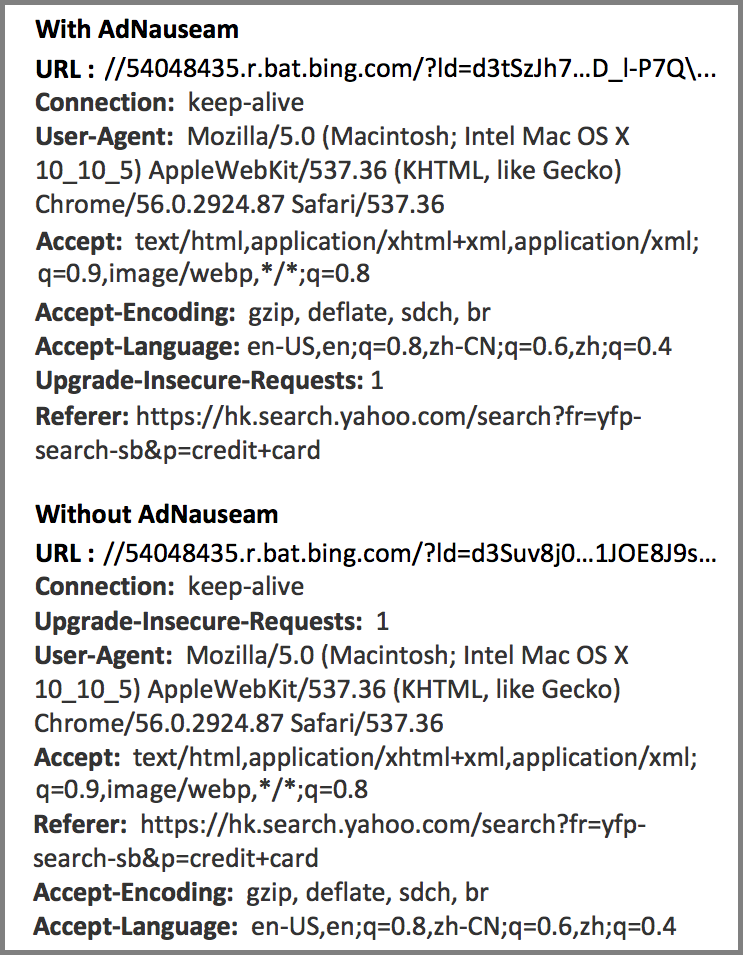
\includegraphics[width=2.5in]{images/headers.png}
% \caption{Header Comparison: AdNauseam click vs. manual request}
% \label{fig:headers}
% \end{figure}

\subsubsection{Comparative}

To further evaluate performance we compare AdNauseam with other commonly used blockers on a range of dimensions, relating both to protection (number of 3rd parties contacted) and usability (page-load speed and memory efficiency) Tests were first run without any extension, then with AdNauseam, Adblock Plus \cite{AdBlock}, uBlock-Origin \cite{Gorhill}, and Privacy Badger \cite{EFF-0}. Tests were performed with each extension's default settings after resetting the browser to its install state. After visiting the websites in the test set (between 15 and 85 popular URLs, depending on the test) via the Selenium browser automation tool, we evaluated the safety of each extension in terms of the number of 3rd parties contacted (Figure \ref{fig:thirdparty}), memory efficiency (Figure \ref{fig:memory}), and page-load speed (Figure \ref{fig:loadtime}). As shown in the graphs below, AdNauseam performed better on all dimensions than no blocker and, perhaps surprisingly, better than AdBlock Plus. As expected, AdNauseam performed less well than uBlock, due to the need to allow visual ad resources, rather than blocking them outright. Privacy Badger varied according to the test in question and on whether it had been pre-trained.

\begin{figure}[!t]
\centering
\includegraphics[width=2.5in]{images/thirdparty.png}
\caption{Number of distinct third-parties contacted.}
\label{fig:thirdparty}
\vspace{6mm}
\includegraphics[width=2.5in]{images/memory.png}
\caption{Overall memory footprint (MB).}
\label{fig:memory}
\vspace{6mm}
\includegraphics[width=2.5in]{images/loadtime.png}
\caption{Total page load time (sec).}
\label{fig:loadtime}
\end{figure}


\subsection{Ethical}

In adopting the philosophy of data obfuscation AdNauseam seeks to shields users from the inexorable, and inappropriate probes of services and third parties. Choosing obfuscation, however, means taking seriously the ethical critiques that it has drawn, including charges that it is dishonest, wastes resources, and pollutes data repositories. Addressing these issues in \emph{Obfuscation: A User's Guide to Privacy and Protest} \cite{Brunton}, the authors charge creators of obfuscating systems to answer two questions: first, whether their aims are laudable; and second, whether alternative approaches exist which might achieve these aims at lesser cost. Regarding the first charge we take as a point of departure that ubiquitous online surveillance violates the tenets of a liberal democracy. The troubling nature of this surveillance apparatus is exacerbated by its surreptitious operation, its prevarication, and its resistance to the wishes of a majority of users. Others have eloquently established these claims through systems' analysis, demonstrations and public opinion surveys. \cite{Turow, Goldfarb, Tucker} Data generated from online surveillance contributes to the creation of valuable, but often highly problematic profiles that fuel the information and behavioral advertising industries with uncertain, potentially negative effects on their subjects. Against this backdrop, we judge the aims of AdNauseam, which include the disruption of this process, to be morally defensible.

The second charge to designers whether obfuscation impose a lower collateral costs than alternative approaches for achieving similar ends. Comparing the purported cost or damage caused by AdNauseam against alternative approaches involves more measurements and even more uncertainties than we are able to tackle here. But, by the same token, this dearth of concrete evidence also poses a challenge to critics who accuse ad blockers---and would similarly accuse AdNauseam---of harming the web's economy. Even if one holds that the “best” resolution would be societal-level regulation, there has been little progress on this front despite sustained privacy activism. As important as seeking credible alternatives, however, is weighing the purported harms or costs of using AdNauseam. Among the latter, the harm of “wasting” network bandwidth or server resources is ironic at best, given the vast amount of bandwidth used by advertisers and trackers, the performance degradation resulting from loading this unwanted content, and the financial toll on users paying for fixed data plans. From an ethical perspective, it is questionable whether the term “waste” is appropriate at all. For those who deliberately choose to install and use AdNauseam, it offers utility as a protective shield for privacy and an escape from inappropriate profiling. In our view, these are not worthless endeavors.

One of the most aggressive charges leveled at AdNauseam is that it perpetuates “click fraud.” Since obfuscation and fraud both involve forms of lying that disrupt entrenched systems, it is important to evaluate whether the two forms are alike. To carry this out, we consult various definitions: “[Click] fraud occurs when a person, automated script or computer program imitates a legitimate user of a web browser, clicking on such an ad without having actual interest in the target of the ad's link” \cite{Liu} comes close to capturing AdNauseam in its notion of clicking without actual interest, but this definition seemed overly broad in that it commits users to click only on ads in which they are interested, and seems an unjustifiable restriction on liberty of action. We also argue that if the automated script is performing as an agent of an individual, through that individual's legitimate choice, then the script is a proxy for the user. John Battelle's account \cite{Battelle}, which includes motive and intention, gets closer to the standard meaning of “fraud” in “click fraud”: the “‘decidedly black hat’ practice of publishers illegitimately gaming paid search advertising by employing robots or low-wage workers to repeatedly click on each AdSense ad on their sites, thereby generating money to be paid by the advertiser to the publisher and to Google.” While elements of the above definitions overlap with AdNauseam's clicking (without genuine interest in their targets), machine automation is only incidental to click fraud, and may instead involve “low-wage workers.” More significant is what AdNauseam does not share with click fraud, namely action on behalf of stakeholders resulting in financial gain. In litigated cases of click fraud the intention to inflate earnings has been critical.

We readily admit that a primary aim of AdNauseam is to disrupt business models that support surreptitious surveillance. It does not follow however that AdNauseam is responsible for the demise of free content on the web. First, it is not, as we make clear on the project page, advertising that is the primary target of the project, but rather the tracking of users without their consent. Contextual advertising that does not involve tracking can certainly support free content just as it has in the past. Second, web content is not actually ‘free’ as this argument implies. The development of the Internet has been supported largely by government funding (and thus by taxpayers) since its beginning. In fact, vast infrastructure and energy costs are still born in large part by taxpayers, not to mention the potentially species-threatening cost to the environment posed by increasing data traffic \cite{Hazas}. Critics may say that ad blocking users free ride upon those who allow themselves to be tracked, however, in our view this presumes an entitlement on the part of trackers that is indefensible; one may equally charge trackers with destructive exploitation of users \cite{Brunton}. Lastly, in regard to free riding, we wish to point out that the hiding of ads is an optional element of AdNauseam, one that users must explicitly opt into when they install the software (see Figure \ref{fig:firstrun}); AdNauseam's visitation and visualization modules work equally well whether the user elects to view ads or to hide them.

\begin{figure}[!t]
\centering
\includegraphics[width=2.5in]{images/firstrun.png}
\caption{Opt-in settings on initial install page.}
\label{fig:firstrun}
\end{figure}

\section{Related Work}

The strategy of obfuscation has been broadly applied---in search \cite{Howe-1}, location tracking \cite{Meyerowitz}, social networks \cite{Luo}, anonymity \cite{Chakravarty, Schulze}, etc.---and, as such, has been recognized as an important element of the privacy engineer's toolbox. A range of obfuscation-based projects have been described in \cite{Brunton}, including FaceCloak \cite{Luo}, for Facebook profiles, BitTorrent Hydra \cite{Schulze}, for decoy torrent sites, and CacheCloak \cite{Meyerowitz}, for location data. There have also been a number of obfuscation schemes for web search \cite{Gervais}.

Other relevant work, described in \cite{Howe-3}, has come from the art/tech community. “I Like What I See” is a tool  that automatically clicks all ‘Like’ links on Facebook to obscure user interests. “ScareMail” \cite{Grosser}, mentioned above, is an extension built atop Gmail that append an algorithmically-generated narrative containing NSA “trigger-words” to the end of each sent email. “Invisible”\cite{Hagborg} extends obfuscation to the context of genetic privacy via a spray that obfuscates DNA to frustrate identification.

Two early tools addressing surveillance integrate ad-blocking with some broadly-defined social good: AddArt \cite{AddArt} replaces ads with user-configurable art, while AdLiPo \cite{Howe-0} does the same with language art. Lightbeam \cite{Mozilla}, provides displays of users' connections, including to advertising networks (though not ads themselves). Floodwatch \cite{Floodwatch} is the one tool we have found that provide visualizations similar to our own, though it requires communication with one or more 3rd-party servers to do so. Privacy Badger \cite{EFF-0} blocks third-party requests based on real-time monitoring of the connections they attempt rather than via lists, blocking only those resources engaged in tracking.

\section{Future Work}

AdNauseam provides individuals with the means to express their commitment to online privacy without the need to depend on the good will or intervention of third-parties. Although fully functional, AdNauseam is perhaps best considered as a proof of concept for a particular approach to privacy, that is, privacy through obfuscation. As discussed, AdNauseam's potential lies in its capacity to protect individuals against data profiling, as well as simultaneously providing a proactive means of expressing one's views to monolithic and largely uninterested corporations. Going forward, a scientific approach to evaluating AdNauseam's performance, or the performance of any system adopting obfuscation, needs a rigorous means of measuring success---namely, evidence that decoy clicks have been registered and have an impact on the resulting profile. Such needs are likely to turn not only on the statistical analysis of signal-to-noise ratios, but also on a practical understanding of how click data is actually mined and used, and the extent to which it influences aspects of user profiles. This would allow future iterations of obfuscation-based tools to be both effective and efficient in the noise they produce.

More concrete future work could take several directions. In the near term we hope to better answer the question of how to perform indistinguishable clicks without exposing users to potential harms via downloaded content, as discussed above. Though complex, P2P approaches for the sharing of obfuscation data between users is a ripe area of future work, with users potentially visiting the ads detected by peers as a means of both shielding their data and maximizing indistinguishability. A central challenge here would be meeting functional criteria while not compromising the design constraints discussed early in this paper, e.g., transparency and independence from third-parties. Finally, beyond the technical, work exploring the motivations and qualitative experiences of users who select obfuscation tools could shed light on the unique potential such tools might offer in additional domains.


\section{Conclusions}

AdNauseam operates in an environment that is both technologically and socially complex, one in which user data is perceived to be highly valuable. For individuals, however, patterns recorded over time potentially open a window into their lives, interests, and ambitions. Thus surveillance via advertising is not only a source of individual vulnerability, but also interferes with the rights to free and autonomous inquiry, association, and expression that are essential to a healthy democratic society. Consequently, there remain tensions between individual users, collective social and political values, and the economic interests of publishers and advertisers. In a better world, this tension would be resolved in a transparent, trust-based accommodation of respective interests. Instead, concerned users find little transparency and few credible assurances from advertisers that privacy will ever trump the pursuit of profit. Thus trust-based mutual accommodation gives way to an adversarial relationship, one in which we must leverage all the strategies at our disposal. Our success in this endeavor will depend in part on how well we share our experience applying known strategies to new contexts, in concrete and specific detail, according to an evolving set of best practices, as we have attempted above.

We conclude with a philosophical point. In some of the most revealing exchanges we have had with critics, we note a palpable sense of indignation, one that appears to stem from the belief that human users have an \emph{obligation} to remain legible to their systems, a duty to remain trackable. We see things differently; advertisers and service providers are not by default entitled to the externalities of our online activity. Rather, users should control the opacity of their actions, while powerful corporate entities should be held to the highest standards of transparency. Unfortunately this is the opposite of the status quo. The trackers want us to remain machine-readable, so that they can exploit our most human endeavors (sharing, learning, searching, socializing) to extract value and pursue profit. AdNauseam attempts to represent an alternative position.

\section*{Acknowledgements}
The authors with to thank our (anonymous) reviewers for their close-reading and constructive suggestions on the original draft of this paper. We also thank Mushon Zer-Aviv, for his generous contributions to all aspects of the project.  This publication has been supported in part by a grant from the Research Grants Council of the Hong Kong Special Administrative Region, China (Project No. CityU 11669616)


\begin{thebibliography}{99}

\bibitem{AdBlock} AdBlock Plus. “AdBlock Plus.” n.d. https://adblockplus.org/.

\bibitem{AddArt} AddArt. “AddArt.” n.d. http://add-art.org/.

\bibitem{Battelle} Battelle, John. \textit{ The Search: How Google and Its Rivals Rewrote the Rules of Business and Transformed Our Culture}. Nicholas Brealey Publishing, 2011.

\bibitem{Brunton} Brunton, Finn, and Helen Nissenbaum. \textit{Obfuscation: A User's Guide for Privacy and Protest}. MIT Press, 2015.

\bibitem{Cavoukian} Cavoukian, Ann, and Michelle Chibba. “Cognitive Cities, Big Data and Citizen Participation: The Essentials of Privacy and Security”. \textit{Towards Cognitive Cities}. Springer International Publishing, 2016. 61-82.

\bibitem{ClickFraud} Click Fraud. (n.d.). In Wikipedia. Retrieved August 1, 2016. https://en.wikipedia.org/wiki/Click\_fraud

\bibitem{Chakravarty} Chakravarty, Sambuddho, et al. “Detecting Traffic Snooping in Anonymity Networks Using Decoys.” (2011).

\bibitem{EasyList} “EasyList.” 2016. https://easylist.to/

\bibitem{Englehardt} Englehardt, Steven, and Arvind Narayanan. “Online Tracking: A 1-million-site Measurement and Analysis.” \textit{Proceedings of the 2016 ACM SIGSAC Conference on Computer and Communications Security}. ACM, 2016.

\bibitem{EFF-0} Electronic Frontier Foundation. “Privacy Badger.”\\n.d. https://www.eff.org/privacybadger.
\bibitem{EFF-1} Electronic Frontier Foundation. “Do Not Track.”\\n.d. https://www.eff.org/issues/do-not-track.

\bibitem{Flanagan} Flanagan, Mary, Daniel C. Howe, and Helen Nissenbaum. “Embodying Values in Technology: Theory and Practice.” \textit{Information technology and moral philosophy}. (2008): 322-353.

\bibitem{Floodwatch} Floodwatch. “Floodwatch.” n.d. https://floodwatch.o-c-r.org/.

\bibitem{Friedman} Friedman, Batya, Daniel C. Howe, and Edward Felten. “Informed Consent in the Mozilla Browser: Implementing Value-Sensitive Design”. \textit{Proceedings of the 35th Annual Hawaii International Conference on System Sciences}. IEEE, 2002.

\bibitem{Gervais} Gervais, Arthur, et al. “Quantifying Web-Search Privacy.” \textit{Proceedings of the 2014 ACM SIGSAC Conference on Computer and Communications Security}. ACM, 2014.

\bibitem{Goldfarb} Goldfarb, Avi, and Catherine Tucker. “Shifts in Privacy Concerns.” \textit{The American Economic Review} 102.3 (2012): 349-353.

\bibitem{Gorhill} Gorhill. “uBlock Origin - An efficient blocker for Chromium and Firefox.” 2016. https://github.com/gorhill/uBlock

\bibitem{Grosser} Grosser, Ben. “ScareMail.” 2013.\\ Web http://bengrosser.com/projects/scaremail/.

\bibitem{Gurses-0} G\"urses, Seda, Carmela Troncoso, and Claudia Diaz. “Engineering Privacy by Design.” \textit{Computers, Privacy \& Data Protection} 14.3 (2011).

\bibitem{Gurses-1} G\"urses, Seda, Carmela Troncoso, and Claudia Diaz. “Engineering Privacy by Design Reloaded.” \textit{Amsterdam Privacy Conference}. 2015.

\bibitem{Hagborg} Dewey-Hagborg, H. ``Invisible.'' 2014. \\ http://www.newmuseumstore.org/browse.cfm/invisible/4,6471.html.

\bibitem{Hansen} Hansen, Marit, Meiko Jensen, and Martin Rost. “Protection Goals for Privacy Engineering.” \textit{Security and Privacy Workshops (SPW)}. IEEE, 2015.

\bibitem{Hazas} Hazas, Mike, et al. “Are there limits to growth in data traffic?: On time use, data generation and speed.” \textit{Proceedings of the Second Workshop on Computing within Limits}. ACM, 2016.

\bibitem{Hoepman} Hoepman, Jaap-Henk. “Privacy Design Strategies.” \textit{IFIP International Information Security Conference}. Springer Berlin Heidelberg, 2014.

\bibitem{Howe-0} Howe, Daniel C. “AdLiPo” 2014. http://rednoise.org/adlipo/.

\bibitem{Howe-1} Howe, Daniel C. and Helen Nissenbaum. “TrackMeNot: Resisting Surveillance in Web Search.” \textit{Lessons from the Identity Trail: Anonymity, Privacy and Identity in a Networked Society} 23 (2009): 417-436.

\bibitem{Howe-3} Howe, Daniel C. “Surveillance Countermeasures: Expressive Privacy via Obfuscation”. APRJA, A Peer-Reviewed Journal About Datafied Research 4.1 (2015).

\bibitem{Iachello} Iachello, Giovanni, and Gregory D. Abowd. “Privacy and Proportionality: Adapting Legal Evaluation Techniques to Inform Design In Ubiquitous Computing.” \textit{Proceedings of the SIGCHI conference on Human factors in computing systems}. ACM, 2005.

\bibitem{Liu} Liu, De, Jianqing Chen, and Andrew B. Whinston. “Current Issues in Keyword Auctions”. \textit{Business Computing (Handbooks in Information Systems, Vol. 3)} (2009): 69-97.

\bibitem{Luo} Luo, Wanying, Qi Xie, and Urs Hengartner. “FaceCloak: An Architecture for User Privacy on Social Networking Sites” \textit{International Conference on Computational Science and Engineering}, 2009.

\bibitem{Mansfield} Mansfield-Devine, Steve. “When advertising turns nasty”. \textit{Network Security} 2015.11 (2015): 5-8.

\bibitem{Meyerowitz} Meyerowitz, Joseph and Romit Roy Choudhury. “Hiding stars with fireworks: Location privacy through camouflage.” \textit{Proceedings of the 15th annual international conference on Mobile computing and networking}. ACM, 2009.

\bibitem{Mozilla} Mozilla. “Lightbeam.” 2016. https://www.mozilla.org/en-US/lightbeam/.

\bibitem{Murphy} Murphy, Kate. “The Ad Blocking Wars.” \textbf{\textit{The New York Times}}, 20 Feb. 2016.

\bibitem{Nikiforakis} Nikiforakis, Nick, et al. “Cookieless monster: Exploring the ecosystem of web-based device fingerprinting.” \textit{IEEE symposium on Security and privacy (SP)}. IEEE, 2013.

\bibitem{Nissenbaum} Nissenbaum, Helen. \textit{Privacy in Context: Technology, Policy and the Integrity of Social Life.} Palo Alto: Stanford University Press, 2010.

\bibitem{PageFair} PageFair, Adobe “The cost of ad blocking–PageFair and Adobe 2015 Ad Blocking Report (2015).”

% \bibitem{Peddinti} Peddinti, Sai Teja, and Nitesh Saxena. “On the Privacy of Web Search Based on Query
% Obfuscation: A Case Study of TrackMeNot.” \textit{International Symposium on Privacy Enhancing Technologies Symposium}. Springer Berlin Heidelberg, 2010.

\bibitem{Regan} Regan, Priscilla M. \textit{Legislating privacy: Technology, social values, and public policy.} Univ of North Carolina Press, 1995.

\bibitem{Schulze} Schulze, Hendrik, and Klaus Mochalski. “Internet Study 2008/2009.” \textit{Ipoque Report} 37 (2009): 351-362.

\bibitem{Spiekermann} Spiekermann, Sarah, and Lorrie Faith Cranor. “Engineering Privacy.” \textit{IEEE Transactions on software engineering} 35.1 (2009): 67-82.

\bibitem{Tucker} Tucker, Catherine E. “Social networks, personalized advertising, and privacy controls.” \textit{Journal of Marketing Research} 51.5 (2014): 546-562.

\bibitem{Turow} Turow, Joseph, et al. “Americans reject tailored advertising and three activities that enable it.” (2009).

\bibitem{Wills} Wills, Craig E., and Doruk C. Uzunoglu. “What Ad Blockers Are (and Are Not) Doing." \textit{Fourth IEEE Workshop on Hot Topics in Web Systems and Technologies (HotWeb)}. IEEE, 2016.


\end{thebibliography}

\end{document}
